% Gemini theme
% https://github.com/anishathalye/gemini

\documentclass[final]{beamer}

% ====================
% Packages
% ====================

\usepackage[T1]{fontenc}
\usepackage{lmodern}
\usepackage[size=custom,width=70,height=100,scale=0.963]{beamerposter}
% \usepackage[size=custom,width=70,height=100,scale=0.9]{beamerposter}
\usetheme{gemini}
\usecolortheme{gemini}
\usepackage{graphicx}
\usepackage{booktabs}
\usepackage{tikz}
\usepackage{pgfplots}
\pgfplotsset{compat=1.14}
\usepackage{anyfontsize}
% \usepackage{pgfplotstable}
% \usepackage{soul}

\usepackage{kinematikz} %requires TeX Live 2022!!
\usetikzlibrary{arrows.meta}
\usetikzlibrary{shapes,arrows,positioning,calc}
\usetikzlibrary{positioning,backgrounds,patterns}
\usetikzlibrary{decorations.pathreplacing}
\usetikzlibrary{shapes.geometric}
% \sisetup{ detect-family = true, } %to allow sans-serif in math mode units
\usepackage{ifthen}
\usetikzlibrary{matrix,calc}

\usepgfplotslibrary{groupplots}
\usepgfplotslibrary{fillbetween} 
\usepgfplotslibrary{units}

\newcommand{\graphLineWidth}{0.4mm}
\newcommand{\pullColor}{red}
\newcommand{\pushColor}{blue}
\newcommand{\shakeColor}{green}
\newcommand{\twistColor}{orange}
\newcommand{\actionOpacity}{0.10}
% A base color for the confusion matrix
\definecolor{cfcolor}{HTML}{042D6E}
\usepackage{svg}

%Adjust these definitions for adequate consistency in the text. This is an example. You can adjust for better typesetting!
\newcommand{\pull}{\textsc{pull}}
\newcommand{\push}{\textsc{push}}
\newcommand{\shake}{\textsc{shake}}
\newcommand{\twist}{\textsc{twist}}

\let\comment\undefined % because someone else defines it (amsmath, verbatim, anyone else ...?)
% \usepackage[commandnameprefix=ifneeded]{changes}
% \usepackage[final]{changes} % for the final acceptance of all changes
% \usepackage{enumitem}
\tikzset{
   vsblack/.style={
   black, %force black color override the elsevier template inside tikz figures and plots. Comment this line not to override!
   }, 
}

% ====================
% Lengths
% ====================

% If you have N columns, choose \sepwidth and \colwidth such that
% (N+1)*\sepwidth + N*\colwidth = \paperwidth
\newlength{\sepwidth}
\newlength{\colwidth}
\setlength{\sepwidth}{0.025\paperwidth}
\setlength{\colwidth}{0.3\paperwidth}

\newcommand{\separatorcolumn}{\begin{column}{\sepwidth}\end{column}}

% ====================
% Title
% ====================

\title{Domain Adaptation with Contrastive Simultaneous Multi-loss
Training for Hand Gesture Recognition}

\author{Joel Baptista \inst{1} \and Vítor Santos \inst{1} \and Filipe Silva \inst{1} \and Diogo Pinho \inst{2}}

\institute[shortinst]{\inst{1} Institute of Electronics and Informatics Engineering of Aveiro (IEETA) \samelineand \\ \inst{2} Bosch Termotecnologia, S. A.  }

% ====================
% Footer (optional)
% ====================

\footercontent{
  \href{https://doi.org/10.3390/s23063332}{https://doi.org/10.3390/s23063332} \hfill
  \hfill
  \href{mailto:joelbaptista@ua.pt}{joelbaptista@ua.pt}}
% (can be left out to remove footer)

% ====================
% Logo (optional)
% ====================

% use this to include logos on the left and/or right side of the header:
\logoright{
\includegraphics[height=10cm, trim={0 0.5cm 0 0}, clip]{img/Ciencia_2024_Horizontal_Branco.png}}
% \logoright{
\includegraphics[height=1cm]{img/Ciencia_2024_Horizontal_Branco.png}}
\logoleft{
\includegraphics[height=9cm, trim={0 0.0 12cm 0}, clip]{img/ieeta.png}}

% ====================
% Body
% ====================

\begin{document}

\begin{frame}[t]
\begin{columns}[t]
\separatorcolumn

\begin{column}{\colwidth}

  \begin{block}{Introduction}


    Hand gestures are an important aspect of human communication, serving several purposes 
    such as enhancing spoken messages, signaling intentions or expressing emotions. 
    Driven by technological advances, the process of classifying meaningful hand gestures, 
    known as Hand Gesture Recognition (HGR), has received increasing attention in recent years.
    
    The major application areas of gesture recognition include sign language translation, 
    human-machine interaction, medical rehabilitation, and virtual reality. HGR systems also 
    target robotic applications using a variety of input devices, among which stands out color
    cameras, depth sensors or gloves with embedded sensors. In this context, the ability of 
    robots to recognize hand gestures
    seems very promising for progress in Human-Robot Collaboration (HRC), 
    as these gestures are simple and intuitive for a human partner to produce. This, in turn, allows 
    humans and robots to coexist and cooperate, improving task efficiency and safety.


    However, HGR is an inherently challenging task due to the complex, non-rigid properties of the hand, 
    such as its shape, color, and orientation. Vision-based HGR systems must also be robust to variations 
    in lighting conditions, cluttered environments, complex backgrounds, and occlusions. In reality, the
    assumption that the training and test datasets are drawn from the same distribution rarely holds in
    practical situations due to domain shifts.
    
    To tackle this issue, this paper proposes a domain adaptation technique for hand gesture recognition in 
    human-robot collaboration scenarios. The proposed approach is based on a two-headed 
    deep architecture that simultaneously adopts cross-entropy and a contrastive loss from
    different network branches to classify hand gestures.

  \end{block}

  \begin{block}{Objectives}

    The main goal is to shed light on the impact of supervised contrastive learning (SCL) 
    on the generalization ability of a trained deep model in gesture classification when faced with a distribution shift.
    For this purpose, the study:

    \begin{itemize}
      \item Contributes with a new RGB annotated dataset of hand gestures, with a complex background 
      and multiple subjects.
      \item Compares the results from the proposed approach against baselines.
    \end{itemize}

  \end{block}

  \begin{block}{Dataset Description}

    This implementation uses four hand gesture
    classes inspired by American Sign Language; the symbols chosen are the "A", "F", "L" and 
    "Y" signs. These signals have the advantage of being well known symbols with already real
    world applications, implying that they are easy to use. These specific signs were chosen
    also because they are relatively distinct. 

    To test the degree of generalization of the proposed method, two datasets were recorded.
    The first dataset was used to train the classification model. This dataset was recorded by one subject, 
    which can be seen in Figure \autoref{fig:gestures_train}.
    
    \begin{figure}[!ht]
      \centering
      \def\vsTW{0.2\textwidth}  %was 0.15\textwidth
      \setlength{\tabcolsep}{2pt} %to make a shorter separation
      \newcommand{\vsTE}[1]{\includegraphics[width=\vsTW]{gestures/#1.png}}
      \begin{tabular}{cccc}
      A & F & L & Y \\
      \vsTE{A1} & \vsTE{F1} & \vsTE{L1} & \vsTE{Y1} \\
      \vsTE{A2} & \vsTE{F2} & \vsTE{L2} & \vsTE{Y2} \\
      \end{tabular}
      \caption{Examples of the training dataset of the four hand gesture classes in the unstructured environment and complex background.
      }
      \label{fig:gestures_train}
    \end{figure}


  \end{block}


\end{column}

\separatorcolumn

\begin{column}{\colwidth}

  \vspace{1.5cm}
  \justify

  The second dataset is used to test the model. This multi-user test dataset was recorded with three subjects
  who were not included in the training dataset. The dataset was recorded on a different day and at a 
  different time of day, resulting in variation in luminosity. Figure 2 shows 
  some samples that constitute the multi-user test dataset.
  
  \begin{figure}[!ht]
    \justify
    \centering
    \def\vsTW{0.2\textwidth}  %was 0.15\textwidth
    \setlength{\tabcolsep}{2pt} %to make a shorter separation
    \newcommand{\vsTE}[1]{\includegraphics[width=\vsTW]{gestures/#1.png}}
    \begin{tabular}{cccc}
    A & F & L & Y \\
    \vsTE{MU_A2} & \vsTE{MU_F2} & \vsTE{MU_L2} & \vsTE{MU_Y2} \\
    \vsTE{MU_A3} & \vsTE{MU_F3} & \vsTE{MU_L3} & \vsTE{MU_Y3} \\
    \end{tabular}
    \caption{Examples of the test dataset with three different subjects and acquired in a different time of day in relation to the training dataset.\label{fig:gestures_test}}
  \end{figure}
  
  Table \autoref{tab:dataset} shows the distribution of samples among all classes. Although the dataset is small
  when compared to the large-scale datasets, it has a distribution of samples per class similar to other 
  static hand gesture datasets used in HGR. Additionally, we apply online data augmentation in the training phase that further help
  compensate for the reduced number of samples. 
 
  \begin{table}[!ht] 
    \centering
    %\newcolumntype{C}{>{\centering\arraybackslash}X}
    \begin{tabular}{lccccc}
      \toprule
      \textbf{Dataset}	& \textbf{A}	& \textbf{F} & \textbf{L} & \textbf{Y} & \textbf{Total}\\
      \midrule
      Training dataset & \num{6430} & \num{6148} & \num{5989} & \num{6044} & \textbf{\num{24611}}\\
      
      Multi-user test dataset & \num{4183} & \num{4277} & \num{4276} & \num{4316} & \textbf{\num{17051}}\\
      \bottomrule
    \end{tabular}
    \caption{Number of images, per class, of the training dataset and the multi-user test dataset. The training dataset includes one subject and the test dataset includes three subjects.\label{tab:dataset}}
    % \noindent{\footnotesize{\textsuperscript{1} Tables may have a footer.}}
  \end{table}

  Both of the datasets were recorded in the collaborative cell located in 
  the Laboratory of Automation and Robotics at the University of Aveiro.

  \begin{block}{Methodology}

    This section describes the proposed contrastive domain adaptation technique for HGR. 
    Our goal is to train a model on the source domain and, then, use it to make
    predictions on the target domain that has different characteristics, namely, different subjects
    and illumination conditions. We compare this approach with traditional transfer learning methods, that 
    consists of the Inception-v3 pre-trained model that is repurposed
    for the specific hand gesture classification task involving four classes.

    SCL has been shown to be effective for domain adaptation, 
    because it can help the model to learn features that are invariant to domain shifts.
    
    The idea behind the proposed contrastive domain adaptation technique is to use a network that 
    branches twice after the encoder model (dual-branch head), allowing to train the representation 
    model and the classification model simultaneously. Figure \autoref{fig:multi_loss} shows the model architecture.

    \begin{figure}[!ht]
      \centering
      % \begin{center}
\begin{tikzpicture}[vsblack]
    \begin{groupplot}[
    group style={group name=training curves,
                group size=2 by 2,
                vertical sep=0.2cm,
                horizontal sep=1.5cm,
                }, 
    height={6 cm},
    % width={ \textwidth / 2 - 10},  
    width={0.50\textwidth-2pt},  
    xmajorgrids=true,
    ymajorgrids=true,
    grid style=dashed,
    ]
    
    % (1, 2) Accuracy
    \nextgroupplot [
        title={Model Cross Entropy Loss},
        ylabel={Loss},
        %ymin=-1, ymax=22,,
        %ytick={0, 5, 10, 15, 20},
        xlabel={Epochs},
        %xmin=-5, xmax=305,
        %xtick={0, 50, 100, 150, 200, 250, 300},
        legend pos=north east,
    ]
    
    \addplot[color=denim, line width = \graphLineWidth]
    table[x=epoch,y= train_loss,col sep=comma]{plots/data/InceptionV3_multi_loss_train.csv};
    
    \addplot[color=deepsaffron, line width = \graphLineWidth]
    table[x=epoch,y= val_loss,col sep=comma]{plots/data/InceptionV3_multi_loss_train.csv};
    
    \legend{Training, Validation}

    % (1, 3) Accuracy
    \nextgroupplot [
        title={Model Contrastive Loss},
        ylabel={Loss},
        %ymin=-1, ymax=22,,
        %ytick={0, 5, 10, 15, 20},
        xlabel={Epochs},
        %xmin=-5, xmax=305,
        %xtick={0, 50, 100, 150, 200, 250, 300},
        legend pos=north east,
    ]
    
    \addplot[color=denim, line width = \graphLineWidth]
    table[x=epoch,y= train_con_loss,col sep=comma]{plots/data/InceptionV3_multi_loss_train.csv};
    
    \addplot[color=deepsaffron, line width = \graphLineWidth]
    table[x=epoch,y= val_con_loss,col sep=comma]{plots/data/InceptionV3_multi_loss_train.csv};
    
    \legend{Training, Validation}

    \end{groupplot}
    % put all plots in same tikzpicture
\begin{axis}[
    title={Model Accuracy},
    yshift=-0.35\columnwidth, % <-- added
    scale only axis=true,
    xlabel = {Epochs},
    ylabel = {Accuracy},
    width=0.76\columnwidth+0.12\textwidth,  % modified 
    height=0.253125\columnwidth,
    % height={8 cm},
    % width={ \textwidth / 2 - 10},  
    xmajorgrids=true,
    ymajorgrids=true,
    grid style=dashed,
     legend pos= south east,
    ytick distance=0.05,
    % grid = both
    ]

    %     % (1, 1) Accuracy
    % \nextgroupplot [
    %     title={Model Accuracy},
    %     ylabel={Accuracy},
    %     %ymin=0.6, ymax=1,
    %     %ytick={0.6, 0.65, 0.70, 0.75, 0.80, 0.85, 0.90, 0.95},
    %     ytick distance=0.05,
    %     xlabel={Epochs},
    %     width={\textwidth-2pt},  
    %     %xmin=-5, xmax=305,
    %     %xtick={0, 50, 100, 150, 200, 250, 300},
    %     legend pos=south east,
    %     y tick label style=
    %     {
    %          /pgf/number format/.cd,
    %          fixed, fixed zerofill,
    %          precision=2
    %     },
    % ]

    \addplot[color=denim, 
    line width = \graphLineWidth
    ]
    table[x=epoch,y= train_acc,col sep=comma]{plots/data/InceptionV3_multi_loss_train.csv};
    
    \addplot[color=deepsaffron, line width = \graphLineWidth]
    table[x=epoch,y= val_acc,col sep=comma]{plots/data/InceptionV3_multi_loss_train.csv};

    \legend{Training, Validation}
    
\end{axis}

    
% \end{groupplot}
\end{tikzpicture}
\end{center}
      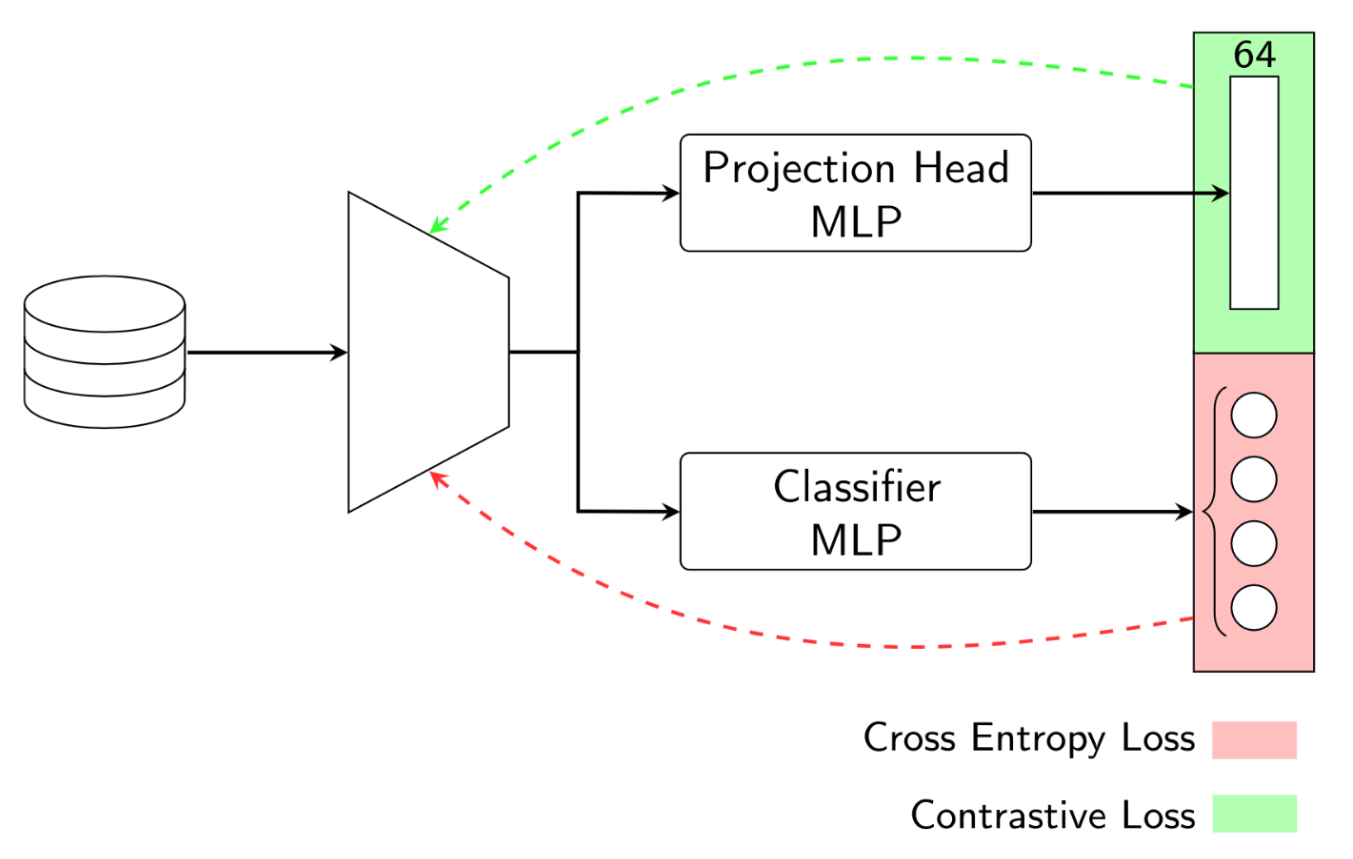
\includegraphics[width=\textwidth]{img/architecture.png}
      \caption{Model's architecture. The losses used are the contrastive loss and the Cross Entropy Loss. \label{fig:multi_loss}}
    \end{figure} 

  \end{block}

\end{column}

\separatorcolumn

\begin{column}{\colwidth}

  \begin{exampleblock}{Contrastive Learning}

    In Contrastive Learning we use a contrastive loss, defined by:

    \begin{equation}
      C_{loss} = \sum_{i \in B} \frac{-1}{p} \sum_{j \in P(i)} \log \frac{e^{(v_i \cdot v_j) / \tau}}{\sum\limits_{a \in A(i)} e^{(v_i \cdot v_a) / \tau}}
      \label{eq:con_loss}\text{,}
    \end{equation}

    This loss function encourages the base model to produce
    similar feature vectors in the same class and dissimilar feature vectors in 
    different classes.

    \heading{Variables}

    Each batch $B$ has $v_i$ feature vectors. The set $P(i)$ 
    represents the indexes of the positive samples $j$ in relation to an anchor 
    sample $i$, and it has a size of $p$. A sample is classified as positive when 
    it belongs to the same class as the anchor. The set $A(i)$ includes all
    the indexes of $B$ except $i$. The exponents exhibit the dot product between 
    two feature vectors divided by a scalar temperature parameter $\tau$.

  \end{exampleblock}
  \begin{block}{Results}

    \def\globalCMscale{1.9}
    % \begin{figure}[!ht]
    %   \centering
    %   %The matrix in numbers. Adjust to your needs :-)
\def\myConfMat{{
{66.5, 2.8, 6.6,  24.2},  %row 1
{ 0.2,80.3, 7.1,  12.4},  %row 2
{ 0.1, 1.0,98.4,  0.6},  %row 3
{ 0.1, 2.3,6.2, 91.5},  %row 4
}}
%
\def\classNames{{"A","F","L","Y"}} %class names. Adapt at will
%
\def\numClasses{4} %number of classes. Could be automatic, but you can change it for tests.
%
\ifthenelse{\isundefined{\globalCMscale}}
{
\def\myScale{2} % 1.5 is a good scale. Values under 1 may need smaller fonts! _vs changed scale to 1.25 since 1.65 seems too large... and we need to save space :-)
}
{\def\myScale{\globalCMscale}} %use a global scale in the document if it is defined
\begin{tikzpicture}[
    vsblack,
    scale = \myScale,
    font={\small}, %for smaller scales, even \tiny may be useful
    ]
%
\tikzset{vertical label/.style={rotate=90,anchor=east}}   % usable styles for below
\tikzset{diagonal label/.style={rotate=45,anchor=north east}}

\foreach \y in {1,...,\numClasses} %loop vertical starting on top
{
    % Add class name on the left
    \node [anchor=east] at (0.4,-\y) {\pgfmathparse{\classNames[\y-1]}\pgfmathresult}; 
    
    \foreach \x in {1,...,\numClasses}  %loop horizontal starting on left
    {
%---- Start of automatic calculation of totSamples for the column ------------   
    \def\totSamples{0}
    \foreach \ll in {1,...,\numClasses}
    {
        \pgfmathparse{\myConfMat[\x-1][\ll-1]}   %fetch next element
        \xdef\totSamples{\totSamples+\pgfmathresult} %accumulate it with previous sum
        %must use \xdef fro global effect otherwise lost in foreach loop!
    }
    \pgfmathparse{\totSamples} \xdef\totSamples{\pgfmathresult}  % put the final sum in variable
%---- End of automatic calculation of totSamples ----------------
 %   
    \begin{scope}[shift={(\x,-\y)}]
        \def\mVal{\myConfMat[\y-1][\x-1]} % The value at index y,x (-1 because of zero indexing)
%        \pgfmathtruncatemacro{\r}{\mVal}   %
        \pgfmathsetmacro{\r}{\mVal} % the absolute value
        \pgfmathsetmacro{\p}{\r/\totSamples*100}  %the percentual value
        \pgfmathtruncatemacro{\pr}{round(\r/\totSamples*100)}  % A rounded percentage to units for aux calc
        \coordinate (C) at (0,0);
        \ifthenelse{\pr<50}{\def\txtcol{black}}{\def\txtcol{white}} %decide text color for contrast
        \node[
            draw,                 %draw lines
            text={\txtcol},         %text color (automatic for better contrast)
            align=center,         %align text inside cells (also for wrapping)
            fill=cfcolor!\pr,        %intensity of fill (can change base color)
            minimum size=\myScale*10mm,    %cell size to fit the scale and integer dimensions (in cm)
            inner sep=0,          %remove all inner gaps to save space in small scales
            ] (C) {
            %Next lines can used/adapted for dual representations of data (total and calculated percentage...)
            \pgfkeys{/pgf/number format/.cd,fixed,fixed zerofill,precision=2}
            \r%\%
%			\\\pgfmathprintnumber{\p}\%
%%            \p\%
            };     %text to put in cell (adapt at will)
        %Now if last vertical class add its label at the bottom
        \ifthenelse{\y=\numClasses}{
        \node [] at ($(C)-(0,0.75)$) % can use vertical or diagonal label as option
        {\pgfmathparse{\classNames[\x-1]}\pgfmathresult};}{}
    \end{scope}
    }
}
%Now add x and y labels on suitable coordinates
\coordinate (yaxis) at (-0.3,0.5-\numClasses/2);  %must adapt if class labels are wider!
\coordinate (xaxis) at (0.5+\numClasses/2, -\numClasses-1.25); %id. for non horizontal labels!
\node [vertical label,yshift=0pt] at (yaxis) {True Label}; % 0pt instead of 16pt _vs
\node []               at (xaxis) {Predicted Label};
\end{tikzpicture}%
    %   % %The matrix in numbers. Adjust to your needs :-)
\def\myConfMat{{
{50.35, 6.29, 0.54,  42.81},  %row 1
{ 0.00,85.33, 0.65,  14.02},  %row 2
{ 0.00, 6.34,91.27,  2.39},  %row 3
{ 0.00, 5.02,5.46, 89.52},  %row 4
}}
%
\def\classNames{{"A","F","L","Y"}} %class names. Adapt at will
%
\def\numClasses{4} %number of classes. Could be automatic, but you can change it for tests.
\ifthenelse{\isundefined{\globalCMscale}}
{
\def\myScale{1.65} % 1.5 is a good scale. Values under 1 may need smaller fonts! _vs changed scale to 1.25 since 1.65 seems too large... and we need to save space :-)
}
{\def\myScale{\globalCMscale}} %use a global scale in the document if it is defined
\begin{tikzpicture}[
    vsblack,
    scale = \myScale,
    font={\small}, %for smaller scales, even \tiny may be useful
    ]
%
\tikzset{vertical label/.style={rotate=90,anchor=east}}   % usable styles for below
\tikzset{diagonal label/.style={rotate=45,anchor=north east}}
%
\foreach \y in {1,...,\numClasses} %loop vertical starting on top
{
    % Add class name on the left
    \node [anchor=east] at (0.4,-\y) {\pgfmathparse{\classNames[\y-1]}\pgfmathresult}; 
    
    \foreach \x in {1,...,\numClasses}  %loop horizontal starting on left
    {
%---- Start of automatic calculation of totSamples for the column ------------   
    \def\totSamples{0}
    \foreach \ll in {1,...,\numClasses}
    {
        \pgfmathparse{\myConfMat[\x-1][\ll-1]}   %fetch next element
        \xdef\totSamples{\totSamples+\pgfmathresult} %accumulate it with previous sum
        %must use \xdef fro global effect otherwise lost in foreach loop!
    }
    \pgfmathparse{\totSamples} \xdef\totSamples{\pgfmathresult}  % put the final sum in variable
%---- End of automatic calculation of totSamples ----------------
%    
    \begin{scope}[shift={(\x,-\y)}]
        \def\mVal{\myConfMat[\y-1][\x-1]} % The value at index y,x (-1 because of zero indexing)
%        \pgfmathtruncatemacro{\r}{\mVal}   %
        \pgfmathsetmacro{\r}{\mVal} % the absolute value
        \pgfmathsetmacro{\p}{\r/\totSamples*100}  %the percentual value
        \pgfmathtruncatemacro{\pr}{round(\r/\totSamples*100)}  % A rounded percentage to units for aux calc
        \coordinate (C) at (0,0);
        \ifthenelse{\pr<50}{\def\txtcol{black}}{\def\txtcol{white}} %decide text color for contrast
        \node[
            draw,                 %draw lines
            text={\txtcol},         %text color (automatic for better contrast)
            align=center,         %align text inside cells (also for wrapping)
            fill=cfcolor!\pr,        %intensity of fill (can change base color)
            minimum size=\myScale*10mm,    %cell size to fit the scale and integer dimensions (in cm)
            inner sep=0,          %remove all inner gaps to save space in small scales
            ] (C) {
            %Next lines can used/adapted for dual representations of data (total and calculated percentage...)
            \pgfkeys{/pgf/number format/.cd,fixed,fixed zerofill,precision=2}
            \r%\%
%			\\\pgfmathprintnumber{\p}\%
%%            \p\%
            };     %text to put in cell (adapt at will)
        %Now if last vertical class add its label at the bottom
        \ifthenelse{\y=\numClasses}{
        \node [] at ($(C)-(0,0.75)$) % can use vertical or diagonal label as option
        {\pgfmathparse{\classNames[\x-1]}\pgfmathresult};}{}
    \end{scope}
    }
}
%Now add x and y labels on suitable coordinates
\coordinate (yaxis) at (-0.3,0.5-\numClasses/2);  %must adapt if class labels are wider!
\coordinate (xaxis) at (0.5+\numClasses/2, -\numClasses-1.25); %id. for non horizontal labels!
%\node [vertical label,yshift=0pt] at (yaxis) {True Label}; %vs changed 16pt to 0pt
\node []               at (xaxis) {Predicted Label};
\end{tikzpicture}%
    %   %The matrix in numbers. Adjust to your needs :-)
\def\myConfMat{{
{86.1, 3.6, 0.9,  9.4},  %row 1
{ 0.5,83.8, 3.6,  12.1},  %row 2
{ 0.1, 2.0,94.1,  3.8},  %row 3
{ 0.3, 2.0,1.8, 95.9},  %row 4
}}
%
\def\classNames{{"A","F","L","Y"}} %class names. Adapt at will
%
\def\numClasses{4} %number of classes. Could be automatic, but you can change it for tests.
%
\ifthenelse{\isundefined{\globalCMscale}}
{
\def\myScale{1.65} % 1.5 is a good scale. Values under 1 may need smaller fonts! _vs changed scale to 1.25 since 1.65 seems too large... and we need to save space :-)
}
{\def\myScale{\globalCMscale}} %use a global scale in the document if it is defined
\begin{tikzpicture}[
    vsblack,
    scale = \myScale,
    font={\small}, %for smaller scales, even \tiny may be useful
    ]
%
\tikzset{vertical label/.style={rotate=90,anchor=east}}   % usable styles for below
\tikzset{diagonal label/.style={rotate=45,anchor=north east}}
%
\foreach \y in {1,...,\numClasses} %loop vertical starting on top
{
    % Add class name on the left
    \node [anchor=east] at (0.4,-\y) {\pgfmathparse{\classNames[\y-1]}\pgfmathresult}; 
    
    \foreach \x in {1,...,\numClasses}  %loop horizontal starting on left
    {
%---- Start of automatic calculation of totSamples for the column ------------   
    \def\totSamples{0}
    \foreach \ll in {1,...,\numClasses}
    {
        \pgfmathparse{\myConfMat[\x-1][\ll-1]}   %fetch next element
        \xdef\totSamples{\totSamples+\pgfmathresult} %accumulate it with previous sum
        %must use \xdef fro global effect otherwise lost in foreach loop!
    }
    \pgfmathparse{\totSamples} \xdef\totSamples{\pgfmathresult}  % put the final sum in variable
%---- End of automatic calculation of totSamples ----------------
    
    \begin{scope}[shift={(\x,-\y)}]
        \def\mVal{\myConfMat[\y-1][\x-1]} % The value at index y,x (-1 because of zero indexing)
%        \pgfmathtruncatemacro{\r}{\mVal}   %
        \pgfmathsetmacro{\r}{\mVal} % the absolute value
        \pgfmathsetmacro{\p}{\r/\totSamples*100}  %the percentual value
        \pgfmathtruncatemacro{\pr}{round(\r/\totSamples*100)}  % A rounded percentage to units for aux calc
        \coordinate (C) at (0,0);
        \ifthenelse{\pr<50}{\def\txtcol{black}}{\def\txtcol{white}} %decide text color for contrast
        \node[
            draw,                 %draw lines
            text={\txtcol},         %text color (automatic for better contrast)
            align=center,         %align text inside cells (also for wrapping)
            fill=cfcolor!\pr,        %intensity of fill (can change base color)
            minimum size=\myScale*10mm,    %cell size to fit the scale and integer dimensions (in cm)
            inner sep=0,          %remove all inner gaps to save space in small scales
            ] (C) {
            %Next lines can used/adapted for dual representations of data (total and calculated percentage...)
            \pgfkeys{/pgf/number format/.cd,fixed,fixed zerofill,precision=2}
            \r%\%
%			\\\pgfmathprintnumber{\p}\%
%%            \p\%
            };     %text to put in cell (adapt at will)
        %Now if last vertical class add its label at the bottom
        \ifthenelse{\y=\numClasses}{
        \node [] at ($(C)-(0,0.75)$) % can use vertical or diagonal label as option
        {\pgfmathparse{\classNames[\x-1]}\pgfmathresult};}{}
    \end{scope}
    }
}
%Now add x and y labels on suitable coordinates
\coordinate (yaxis) at (-0.3,0.5-\numClasses/2);  %must adapt if class labels are wider!
\coordinate (xaxis) at (0.5+\numClasses/2, -\numClasses-1.25); %id. for non horizontal labels!
%\node [vertical label,yshift=0pt] at (yaxis) {True Label}; %0 pt instead of 16pt _vs
\node []               at (xaxis) {Predicted Label};
\end{tikzpicture}
    %   \caption{Confusion Matrices of results, in percentage (\%), obtained by training all both models with the single user dataset and testing them with the multi-user dataset with different persons not present in the training dataset; the models are: SLT (left), MSMLT (middle) and SMLT (right).}
    %   \label{fig:cm_normal}
    % \end{figure}

    \begin{figure}[!ht]
      \justify
      \centering
      \def\vsTW{0.2\textwidth}  %was 0.15\textwidth
      \setlength{\tabcolsep}{2pt} %to make a shorter separation
      \newcommand{\vsTE}[1]{\includegraphics[width=\vsTW]{gestures/#1.png}}
      \begin{tabular}{cc}
      \hspace{25mm} Baseline & \hspace{17mm} Our Approach \\
      %The matrix in numbers. Adjust to your needs :-)
\def\myConfMat{{
{66.5, 2.8, 6.6,  24.2},  %row 1
{ 0.2,80.3, 7.1,  12.4},  %row 2
{ 0.1, 1.0,98.4,  0.6},  %row 3
{ 0.1, 2.3,6.2, 91.5},  %row 4
}}
%
\def\classNames{{"A","F","L","Y"}} %class names. Adapt at will
%
\def\numClasses{4} %number of classes. Could be automatic, but you can change it for tests.
%
\ifthenelse{\isundefined{\globalCMscale}}
{
\def\myScale{2} % 1.5 is a good scale. Values under 1 may need smaller fonts! _vs changed scale to 1.25 since 1.65 seems too large... and we need to save space :-)
}
{\def\myScale{\globalCMscale}} %use a global scale in the document if it is defined
\begin{tikzpicture}[
    vsblack,
    scale = \myScale,
    font={\small}, %for smaller scales, even \tiny may be useful
    ]
%
\tikzset{vertical label/.style={rotate=90,anchor=east}}   % usable styles for below
\tikzset{diagonal label/.style={rotate=45,anchor=north east}}

\foreach \y in {1,...,\numClasses} %loop vertical starting on top
{
    % Add class name on the left
    \node [anchor=east] at (0.4,-\y) {\pgfmathparse{\classNames[\y-1]}\pgfmathresult}; 
    
    \foreach \x in {1,...,\numClasses}  %loop horizontal starting on left
    {
%---- Start of automatic calculation of totSamples for the column ------------   
    \def\totSamples{0}
    \foreach \ll in {1,...,\numClasses}
    {
        \pgfmathparse{\myConfMat[\x-1][\ll-1]}   %fetch next element
        \xdef\totSamples{\totSamples+\pgfmathresult} %accumulate it with previous sum
        %must use \xdef fro global effect otherwise lost in foreach loop!
    }
    \pgfmathparse{\totSamples} \xdef\totSamples{\pgfmathresult}  % put the final sum in variable
%---- End of automatic calculation of totSamples ----------------
 %   
    \begin{scope}[shift={(\x,-\y)}]
        \def\mVal{\myConfMat[\y-1][\x-1]} % The value at index y,x (-1 because of zero indexing)
%        \pgfmathtruncatemacro{\r}{\mVal}   %
        \pgfmathsetmacro{\r}{\mVal} % the absolute value
        \pgfmathsetmacro{\p}{\r/\totSamples*100}  %the percentual value
        \pgfmathtruncatemacro{\pr}{round(\r/\totSamples*100)}  % A rounded percentage to units for aux calc
        \coordinate (C) at (0,0);
        \ifthenelse{\pr<50}{\def\txtcol{black}}{\def\txtcol{white}} %decide text color for contrast
        \node[
            draw,                 %draw lines
            text={\txtcol},         %text color (automatic for better contrast)
            align=center,         %align text inside cells (also for wrapping)
            fill=cfcolor!\pr,        %intensity of fill (can change base color)
            minimum size=\myScale*10mm,    %cell size to fit the scale and integer dimensions (in cm)
            inner sep=0,          %remove all inner gaps to save space in small scales
            ] (C) {
            %Next lines can used/adapted for dual representations of data (total and calculated percentage...)
            \pgfkeys{/pgf/number format/.cd,fixed,fixed zerofill,precision=2}
            \r%\%
%			\\\pgfmathprintnumber{\p}\%
%%            \p\%
            };     %text to put in cell (adapt at will)
        %Now if last vertical class add its label at the bottom
        \ifthenelse{\y=\numClasses}{
        \node [] at ($(C)-(0,0.75)$) % can use vertical or diagonal label as option
        {\pgfmathparse{\classNames[\x-1]}\pgfmathresult};}{}
    \end{scope}
    }
}
%Now add x and y labels on suitable coordinates
\coordinate (yaxis) at (-0.3,0.5-\numClasses/2);  %must adapt if class labels are wider!
\coordinate (xaxis) at (0.5+\numClasses/2, -\numClasses-1.25); %id. for non horizontal labels!
\node [vertical label,yshift=0pt] at (yaxis) {True Label}; % 0pt instead of 16pt _vs
\node []               at (xaxis) {Predicted Label};
\end{tikzpicture} & %The matrix in numbers. Adjust to your needs :-)
\def\myConfMat{{
{86.1, 3.6, 0.9,  9.4},  %row 1
{ 0.5,83.8, 3.6,  12.1},  %row 2
{ 0.1, 2.0,94.1,  3.8},  %row 3
{ 0.3, 2.0,1.8, 95.9},  %row 4
}}
%
\def\classNames{{"A","F","L","Y"}} %class names. Adapt at will
%
\def\numClasses{4} %number of classes. Could be automatic, but you can change it for tests.
%
\ifthenelse{\isundefined{\globalCMscale}}
{
\def\myScale{1.65} % 1.5 is a good scale. Values under 1 may need smaller fonts! _vs changed scale to 1.25 since 1.65 seems too large... and we need to save space :-)
}
{\def\myScale{\globalCMscale}} %use a global scale in the document if it is defined
\begin{tikzpicture}[
    vsblack,
    scale = \myScale,
    font={\small}, %for smaller scales, even \tiny may be useful
    ]
%
\tikzset{vertical label/.style={rotate=90,anchor=east}}   % usable styles for below
\tikzset{diagonal label/.style={rotate=45,anchor=north east}}
%
\foreach \y in {1,...,\numClasses} %loop vertical starting on top
{
    % Add class name on the left
    \node [anchor=east] at (0.4,-\y) {\pgfmathparse{\classNames[\y-1]}\pgfmathresult}; 
    
    \foreach \x in {1,...,\numClasses}  %loop horizontal starting on left
    {
%---- Start of automatic calculation of totSamples for the column ------------   
    \def\totSamples{0}
    \foreach \ll in {1,...,\numClasses}
    {
        \pgfmathparse{\myConfMat[\x-1][\ll-1]}   %fetch next element
        \xdef\totSamples{\totSamples+\pgfmathresult} %accumulate it with previous sum
        %must use \xdef fro global effect otherwise lost in foreach loop!
    }
    \pgfmathparse{\totSamples} \xdef\totSamples{\pgfmathresult}  % put the final sum in variable
%---- End of automatic calculation of totSamples ----------------
    
    \begin{scope}[shift={(\x,-\y)}]
        \def\mVal{\myConfMat[\y-1][\x-1]} % The value at index y,x (-1 because of zero indexing)
%        \pgfmathtruncatemacro{\r}{\mVal}   %
        \pgfmathsetmacro{\r}{\mVal} % the absolute value
        \pgfmathsetmacro{\p}{\r/\totSamples*100}  %the percentual value
        \pgfmathtruncatemacro{\pr}{round(\r/\totSamples*100)}  % A rounded percentage to units for aux calc
        \coordinate (C) at (0,0);
        \ifthenelse{\pr<50}{\def\txtcol{black}}{\def\txtcol{white}} %decide text color for contrast
        \node[
            draw,                 %draw lines
            text={\txtcol},         %text color (automatic for better contrast)
            align=center,         %align text inside cells (also for wrapping)
            fill=cfcolor!\pr,        %intensity of fill (can change base color)
            minimum size=\myScale*10mm,    %cell size to fit the scale and integer dimensions (in cm)
            inner sep=0,          %remove all inner gaps to save space in small scales
            ] (C) {
            %Next lines can used/adapted for dual representations of data (total and calculated percentage...)
            \pgfkeys{/pgf/number format/.cd,fixed,fixed zerofill,precision=2}
            \r%\%
%			\\\pgfmathprintnumber{\p}\%
%%            \p\%
            };     %text to put in cell (adapt at will)
        %Now if last vertical class add its label at the bottom
        \ifthenelse{\y=\numClasses}{
        \node [] at ($(C)-(0,0.75)$) % can use vertical or diagonal label as option
        {\pgfmathparse{\classNames[\x-1]}\pgfmathresult};}{}
    \end{scope}
    }
}
%Now add x and y labels on suitable coordinates
\coordinate (yaxis) at (-0.3,0.5-\numClasses/2);  %must adapt if class labels are wider!
\coordinate (xaxis) at (0.5+\numClasses/2, -\numClasses-1.25); %id. for non horizontal labels!
%\node [vertical label,yshift=0pt] at (yaxis) {True Label}; %0 pt instead of 16pt _vs
\node []               at (xaxis) {Predicted Label};
\end{tikzpicture} \\
      \end{tabular}
      \caption{Examples of the test dataset with three different subjects and acquired in a different time of day in relation to the training dataset.\label{fig:gestures_test}}
    \end{figure}

    \begin{table}[!ht] 
      \centering
      %\newcolumntype{C}{>{\centering\arraybackslash}X}
      \begin{tabular}{lcccc}
        \toprule
        \textbf{Model}	& \textbf{Accuracy}	& \textbf{Recall} & \textbf{Precision} & \textbf{F1}\\
        \midrule
        Baseline & 84.23	& 84.15 & 86.82 & 84.07\\
        Our approach & \textbf{90.03} & \textbf{89.97} & \textbf{90.96} & \textbf{90.12} \\
        \bottomrule
      \end{tabular}
      \caption{Evaluation metrics for testing the both approaches in the multi-user test dataset. These values are the average of the metrics calculated for each class.\label{tab:metrics}}
      % \noindent{\footnotesize{\textsuperscript{1} Tables may have a footer.}}
      \end{table}

  \end{block}

  \begin{block}{Conclusions}

    The focus of this study was the generalization capacity of the model, which was tested using the multi-user
    test dataset. In this testing phase, the results show that joining cross entropy loss and contrastive loss in a
    multi-loss training approach helps the model reach higher accuracy. In fact, this approach
    performed an increase of 6\% in the accuracy of the model, compared to the traditional transfer learning
    method of training the model only with the CEL. This shows that contrastive learning is
    focused on learning task-specific and invariant features, being more effective to deal with the domain shift
    problem.

  \end{block}


  \begin{block}{References}

    % \nocite{*}
    % \footnotesize{\bibliographystyle{plain}\bibliography{poster}}
    % \begin{thebibliography}{999}

\bibitem[Mohamed(2021)]{Mohamed2021} %01
Mohamed,N.; Mustafa,M.B.; Jomhari,N. A Review of the Hand Gesture Recognition System: Current Progress and Future Directions. {\em IEEE Access} {\bf 2021}, {\em 9}, 157422--157436.

\bibitem[Rautaray(2015)]{Rautaray2015} %02
Rautaray, S.S.; Agrawal, A.  Vision based hand gesture recognition for human computer interaction: a survey. {\em Artificial Intelligence Review} {\bf 2015}

\bibitem[Liu(2018)]{Liu2018} %03
Liu, H.; Wang, L.  Gesture recognition for human-robot collaboration: A review. {\em International Journal of Industrial Ergonomics} {\bf 2018}, {68}

\bibitem[Ajoudani(2018)]{Ajoudani2018} %04
Ajoudani, A.;  Zanchettin, A. M.; Ivaldi, S.; Albu-Schäffer, A.; Kosuge, K.; Khatib, O. Progress and prospects of the human–robot collaboration. {\em AR} {\bf 2018}, {\em 42}, 957--975.

\bibitem[El Zaatari(2019)]{ElZaatari2019} %5
El Zaatari, S.; Marei, M.; Li, W.; Usman, Z. Cobot programming for collaborative industrial tasks: An overview. {\em RAS} {\bf 2019}, {\em 116}, 162--180.

\bibitem[Gualtieri(2021)]{Gualtieri2021} %06
Gualtieri, L.; Rauch, E.; Vidoni, R. Emerging research fields in safety and ergonomics in industrial collaborative robotics: A systematic literature review. {\em RCIM} {\bf 2021}, {\em 67}

\bibitem[Castro(2021)]{Castro2021} %07
Castro, A.; Silva, F.; Santos, V. Trends of human-robot collaboration in industry contexts: Handover, learning, and metrics. {\em Sensors} {\bf 2021}, {\em 21}

\bibitem[Bonci(2021)]{Bonci2021} %08
Bonci,A.; Cheng,P.D.C.; Indri,M.; Nabissi,G.; Sibona,F. Human-robot perception in industrial environments: A survey. {\em Sensors} {\bf 2021}, {\em 21}, 1--29.

\bibitem[Hjorth(2021)]{Hjorth2022} %08
Hjorth, S; Chrysostomou, D. Human–robot collaboration in industrial environments: A literature review on non-destructive disassembly. {\em RCIM} {\bf 2022}, {\em 73}

\bibitem[Neto(2019)]{Neto2019} %09
Neto, P.; Simão,M.; Mendes, N.; Safeea, M. Gesture-based human-robot interaction for human assistance in manufacturing. {\em IJAMT} {\bf 2019}, {\em 101}, 119--135.

\bibitem[AlFarid(2021)]{AlFarid2022} %10
Al Farid,F.; Hashim,N.; Abdullah,J.; Bhuiyan,M.R.; Shahida Mohd Isa, W.N.; Uddin,J.; Haque,M.A.; Husen,M.N. A Structured and Methodological Review on Vision-Based Hand Gesture Recognition System. {\em Journal of Imaging} {\bf 2022}, {\em 8}

\bibitem[Oudah(2020)]{Oudah2020} %11
Oudah,M.; Al-Naji,A.; Chahl,J. Hand Gesture Recognition Based on Computer Vision: A Review of Techniques. {\em Journal of Imaging} {\bf 2020}, {\em 6}

\bibitem[Sarma(2021)]{Sarma2021} %12
Sarma,D.; Bhuyan,M.K. Methods, Databases and Recent Advancement of Vision-Based Hand Gesture Recognition for HCI Systems: A Review. {\em SN Computer Science} {\bf 2021}, {\em 2}

\bibitem[Dignan(2022)]{Dignan2022} %13
Dignan,C.;Perez,E.;Ahmad,I.;Huber,M.;Clark,A. An AI-based Approach for Improved Sign Language Recognition using Multiple Videos. {\em Multimed. Tools Appl.} {\bf 2022}, {\em 81(24)}, 34525--34546.

\bibitem[Subramanian(2022)]{Subramanian2022} %14
Subramanian,B.;Olimov,B.;Naik,S.M.;Kim,S.;Park,K.H.;Kim,J. An integrated mediapipe-optimized GRU model for Indian sign language recognition. {\em Sci. Rep.} {\bf 2022}, {\em 12(1)}

\bibitem[Qi(2021)]{Qi2021} %15
Qi,J.; Xu,K.; Ding,X. Approach to hand posture recognition based on hand shape features for human–robot. {\em Complex and Intelligent Systems} {\bf 2022}, {8}, 2825--2842.

\bibitem[Sarma(2022)]{Sarma2022} %16
Sarma,D.; Bhuyan,M.K. Hand Detection by Two-Level Segmentation with Double-Tracking and Gesture Recognition Using Deep-Features. {\em Sensing and Imaging} {\bf 2022}, {23}

\bibitem[Nuzzi(2019)]{Nuzzi2019} %17
Nuzzi,C.; Pasinetti,S.; Lancini,M.; Docchio,F.,Sansoni, G. Deep learning-based hand gesture recognition for collaborative robots {\em IEEE Instrumentation \& Measurement Magazine} {\bf 2019}

\bibitem[Mujahid(2021)]{Mujahid2021} %18
Mujahid,A.; Awan,M.J.; Yasin,A.; Mohammed,M.A.; Damaševičius, R.; Maskeliūnas,R.; Abdulkareem,K.H. Real-time hand gesture recognition based on deep learning YOLOv3 model. {\em Applied Sciences (Switzerland)} {\bf 2021}, {11}

\bibitem[Deng(2009)]{Deng2009} %19
Deng,J.;Dong,W.;Socher,R.;Li,L.;Kai,L.;Li,F. ImageNet: A large-scale hierarchical image database. {\em 2009 IEEE CVPR} {\bf 2009}, 248–-255

\bibitem[Du(2017)]{Du2017} %20
Du, Y.; Jin, W.; Wei, W.; Hu, Y.; Geng, W.  Surface EMG-based intersession gesture recognition enhanced by deep domain adaptation. {\em Sensors} {\bf 2017}, {17(3)}

\bibitem[Zou(2021)]{Zou2021} %21
Zou, Y.; Cheng, L.  A Transfer Learning Model for Gesture Recognition Based on the Deep Features Extracted by CNN. {\em IEEE Transactions on Artificial Intelligence} {\bf 2021}, {2(5)}

\bibitem[Wu(2021)]{Wu2021} %22
Wu, B.X.; Guang, C.; Zhong, J.P.  Research on Transfer Learning of Vision-based Gesture Recognition. {\em International Journal of Automation and Computing} {\bf 2021}, {18(3)}

\bibitem[Zhang(2022)]{Zhang2022} %23
Zhang, Y.; Wu, L.; He, W.; Zhang, Z.; Yang, C.; Wang, Y., Wang, Y., Tain, K.  An Event-Driven Spatiotemporal Domain Adaptation Method for DVS Gesture Recognition. {\em IEEE Transactions on Circuits and Systems II: Express Briefs} {\bf 2022}, {69(3)}

\bibitem[Wang(2018)]{Wang2018} %24
Wang, M.; Deng, W.  Deep visual domain adaptation: A survey. {\em Neurocomputing} {\bf 2018}, {312}

\bibitem[Yang(2020)]{Yang2020} %25
Yang, Q.; Zhang, Y.; Dai, W.; Jialin, S.  Adversarial Transfer Learning. {\em Transfer Learning} {\bf 2020}

\bibitem[Yasen(2019)]{Yasen2019} %26
Yasen, M.; Jusoh,S. A systematic review on hand gesture recognition techniques, challenges and applications. {\em PeerJ Computer Science} {\bf 2019}

\bibitem[Ryumin(2023)]{Ryumin2023} %27
Ryumin, D.; Ivanko, D.; Ryumina, E. Audio-Visual Speech and Gesture Recognition by Sensors of Mobile Devices {\em Sensors} {\bf 2023}, {23(4)}

\bibitem[Sincan(2020)]{Sincan2020} %28
Sincan, O.M.; Keles, H.Y. AUTSL: A Large Scale Multi-modal Turkish Sign Language Dataset and Baseline Methods {\em CoRR} {\bf 2020}, {abs/2008.00932}

\bibitem[Jiang(2021)]{Jiang2021} %29
Jiang, S.; Sun, B.; Wang, L.; Bai, Y.; Li, K.; Fu, Y. Skeleton Aware Multi-modal Sign Language Recognition {\em CoRR} {\bf 2021}, {abs/2103.08833}

\bibitem[Peral(2022)]{Peral2022} %30
Peral,M.;  Sanfeliu,A.;  Garrell,A. Efficient Hand Gesture Recognition for Human-Robot Interactions. {\em IEEE Robotics and Automation Letters} {\bf 2022}, {\em 7}, 10272--10279.

\bibitem[Lugaresi(2019)]{Lugaresi2019} %31
Lugaresi,C.;  Tang,J.;  Nash,H.;  McClanahan,C.;  Uboweja,E.;  Hays,M.;  Zhang,F.;  Chang,C.;  Yong,M.G.;  Lee,J.;  Chang,W.;  Hua,W.;  Georg,M.;  Grundmann,M. MediaPipe: A Framework for Building Perception Pipelines. {\em CoRR} {\bf 2019}, {abs/1906.08172}

\bibitem[Dang(2022)]{Dang2022} %32
Dang,T.L.; Tran,S.D.; Nguyen,T.H.; Kim,S.; Monet,N. An improved hand gesture recognition system using keypoints and hand bounding. {\em Array} {\bf 2022}, {16}

\bibitem[Verma(2021)]{Verma2021} %33
Verma,M.; Gupta,A.; Vipparthi,S.K. One for All: An End-to-End Compact Solution for Hand Gesture Recognition. {\em CoRR} {\bf 2021}, {\\emabs/2105.07143}

\bibitem[Huang(2021)]{Huang2021} %34
Huang,Y.; Yang,J. A multi-scale descriptor for real time RGB-D hand gesture. {\em Pattern Recognition Letters} {\bf 2021}, {23}, 97--144

\bibitem[Sahoo(2022)]{Sahoo2022} %35
Sahoo,J.P.; Prakash,A.J.; Pławiak,P.; Samantray,S. Real-Time Hand Gesture Recognition Using Fine-Tuned Convolutional Neural Network. {\em Sensors} {\bf 2022}, {22}

\bibitem[Patil(2019)]{Patil2019} %36
Patil,A.R.; Subbaraman,S. Pose invariant hand gesture recognition using two stream transfer learning architecture. {\em IJEAT} {\bf 2019}, {9}, 1771--1777

\bibitem[Pinto(2019)]{Pinto2019} %37
Pinto,R.F.; Borges,C.D.B.; Almeida,A.M.A.; Paula,I.C. Static Hand Gesture Recognition Based on Convolutional Neural Networks. {\em J. Electr. Comput. Eng.} {\bf 2019}, {2019}, 1--12

\bibitem[Khosla(2020)]{Khosla2020} %38
Khosla,P.; Teterwak,P.; Wang,C.; Sarna,A.; Tian,Y.; Isola,P.; Maschinot,A.; Liu,C.; Krishnan,D. Supervised Contrastive Learning. {\em CoRR} {\bf 2020}, {abs/2004.11362}

\bibitem[Gabdrakhmanov(2019)]{Gabdrakhmanov2019} %39
Gabdrakhmanov, L.; Garaev, R.; Razinkov, E. RUSLAN: Russian Spoken Language Corpus for Speech Synthesis {\em arXiv} {\bf 2019}

\bibitem[Ronchetti(2016)]{Ronchetti2016} %40
Ronchetti, F.; Quiroga, F.; Estrebou, C.; Lanzarini, L.; Rosete, A. LSA64: A Dataset of Argentinian Sign Language {\em CACIC} {\bf 2016}

\bibitem[Joze(2018)]{Joze2018} %41
Joze, H.R.V. ; Koller, O. MS-ASL: A Large-Scale Data Set and Benchmark for Understanding American Sign Language {\em CoRR} {\bf 2018}, {1812.01053}

\bibitem[Rato(2022)]{Rato2022} %42
Rato,D.; Oliveira,M.; Santos,V.; Gomes,M.; Sappa,A. A sensor-to-pattern calibration framework for multi-modal industrial collaborative cells. {\em J. Manuf. Syst.} {\bf 2022}, {64}, 497--507

\bibitem[Quigley(2009)]{Quigley2009} %43
Quigley,M.; Conley,K.; Gerkey,B.; Faust,J.; Foote,T.; Leibs,J.; Wheeler,R.; Ng, A. ROS: an open-source Robot Operating System. {\em ICRA Workshop on Open Source Software} {\bf 2009}, {3}

\bibitem[Cubuk(2019)]{Cubuk2019} %44
Cubuk,E.D.;Zoph,B.;Shlens,J.;Le,Q.V. RandAugment: Practical data augmentation with no separate search. {\em CoRR} {\bf 2019}, {abs/1909.13719}

\bibitem[Szegedy(2015)]{Szegedy2015} %45
Szegedy,C.;Vanhoucke,V.;Ioffe,S.;Shlens,J.;Wojna,Z. Rethinking the Inception Architecture for Computer Vision. {\em CoRR} {\bf 2015}, {abs/1512.00567}

\bibitem[He(2015)]{He2015} %46
He, K.;Zhang, X.;Ren, S.;Sun, J. Deep Residual Learning for Image Recognition. {\em CoRR} {\bf CoRR},{\em abs/1512.03385}

\bibitem[Robinson(2020)]{Robinson2020} %47
Robinson, J.;Chuang, C.; Sra, S., Jegelka, S. Contrastive Learning with Hard Negative Samples. {\em CoRR} {\bf 2020}, {abs/2010.04592}

\bibitem[Scalbert(2021)]{Scalbert2021} %47
Scalbert, M.;Vakalopoulou, M.; Couzinié-Devy, Multi-Source domain adaptation via supervised contrastive learning
and confident consistency regularization. {\em CoRR} {\bf 2021}, {abs/2106.16093}

\bibitem[Kingma(2014)]{Kingma2014} %47
Kingma, D.P. ;Ba, J. Adam: A Method for Stochastic Optimization. {\em arXiv} {\bf 2014}



% @article{Du2017,
%    author = {Yu Du and Wenguang Jin and Wentao Wei and Yu Hu and Weidong Geng},
%    doi = {10.3390/s17030458},
%    issn = {14248220},
%    issue = {3},
%    journal = {Sensors (Switzerland)},
%    title = {Surface EMG-based inter-session gesture recognition enhanced by deep domain adaptation},
%    volume = {17},
%    year = {2017},
% }


% @article{Wang2018,
%    author = {Mei Wang and Weihong Deng},
%    doi = {10.1016/j.neucom.2018.05.083},
%    issn = {18728286},
%    journal = {Neurocomputing},
%    title = {Deep visual domain adaptation: A survey},
%    volume = {312},
%    year = {2018},
% }

% @article{Yang2020,
%    author = {Qiang Yang and Yu Zhang and Wenyuan Dai and Sinno Jialin Pan},
%    doi = {10.1017/9781139061773.009},
%    journal = {Transfer Learning},
%    title = {Adversarial Transfer Learning},
%    year = {2020},
% }

% @article{Rautaray2015,
%    author = {Siddharth S. Rautaray and Anupam Agrawal},
%    doi = {10.1007/s10462-012-9356-9},
%    issn = {15737462},
%    issue = {1},
%    journal = {Artificial Intelligence Review},
%    title = {Vision based hand gesture recognition for human computer interaction: a survey},
%    volume = {43},
%    year = {2015},
% }

% @article{Liu2018,
%    author = {Hongyi Liu and Lihui Wang},
%    doi = {10.1016/j.ergon.2017.02.004},
%    issn = {18728219},
%    journal = {International Journal of Industrial Ergonomics},
%    title = {Gesture recognition for human-robot collaboration: A review},
%    volume = {68},
%    year = {2018},
% }

% @article{Du2017,
%    author = {Yu Du and Wenguang Jin and Wentao Wei and Yu Hu and Weidong Geng},
%    doi = {10.3390/s17030458},
%    issn = {14248220},
%    issue = {3},
%    journal = {Sensors (Switzerland)},
%    title = {Surface EMG-based inter-session gesture recognition enhanced by deep domain adaptation},
%    volume = {17},
%    year = {2017},
% }

% @article{Zou2021,
%    author = {Yongxiang Zou and Long Cheng},
%    doi = {10.1109/TAI.2021.3098253},
%    issn = {26914581},
%    issue = {5},
%    journal = {IEEE Transactions on Artificial Intelligence},
%    title = {A Transfer Learning Model for Gesture Recognition Based on the Deep Features Extracted by CNN},
%    volume = {2},
%    year = {2021},
% }

% @article{Wu2021,
%    author = {Bi Xiao Wu and Chen Guang Yang and Jun Pei Zhong},
%    doi = {10.1007/s11633-020-1273-9},
%    issn = {17518520},
%    issue = {3},
%    journal = {International Journal of Automation and Computing},
%    title = {Research on Transfer Learning of Vision-based Gesture Recognition},
%    volume = {18},
%    year = {2021},
% }

% @article{Zhang2022,
%    author = {Yuhan Zhang and Lindong Wu and Weihua He and Ziyang Zhang and Chen Yang and Yaoyuan Wang and Ying Wang and Kun Tian and Jianxing Liao and Ying Yang},
%    doi = {10.1109/TCSII.2021.3108798},
%    issn = {15583791},
%    issue = {3},
%    journal = {IEEE Transactions on Circuits and Systems II: Express Briefs},
%    title = {An Event-Driven Spatiotemporal Domain Adaptation Method for DVS Gesture Recognition},
%    volume = {69},
%    year = {2022},
% }



% % Reference 1
% \bibitem[Author1(year)]{ref-journal}
% Author~1, T. The title of the cited article. {\em Journal Abbreviation} {\bf 2008}, {\em 10}, 142--149.
% % Reference 2
% \bibitem[Author2(year)]{ref-book1}
% Author~2, L. The title of the cited contribution. In {\em The Book Title};  Editor 1, F., Editor 2, A., Eds.;  Publishing House: City, Country, 2007;  pp. 32--58.
% % Reference 3
% \bibitem[Author3(year)]{ref-book2}
% Author 1, A.;  Author 2, B. \textit{Book Title}, 3rd ed.;  Publisher: Publisher Location, Country, 2008;  pp. 154--196.
% % Reference 4
% \bibitem[Author4(year)]{ref-unpublish}
% Author 1, A.B.;  Author 2, C. Title of Unpublished Work. \textit{Abbreviated Journal Name} year, \textit{phrase indicating stage of publication (submitted;  accepted;  in press)}.
% % Reference 5
% \bibitem[Author5(year)]{ref-communication}
% Author 1, A.B. (University, City, State, Country);  Author 2, C. (Institute, City, State, Country). Personal communication, 2012.
% % Reference 6
% \bibitem[Author6(year)]{ref-proceeding}
% Author 1, A.B.;  Author 2, C.D.;  Author 3, E.F. Title of presentation. In Proceedings of the Name of the Conference, Location of Conference, Country, Date of Conference (Day Month Year);  Abstract Number (optional), Pagination (optional).
% % Reference 7
% \bibitem[Author7(year)]{ref-thesis}
% Author 1, A.B. Title of Thesis. Level of Thesis, Degree-Granting University, Location of University, Date of Completion.
% % Reference 8
% \bibitem[Author8(year)]{ref-url}
% Title of Site. Available online: URL (accessed on Day Month Year).
\end{thebibliography}

    \footnotesize

    Rato, D., Oliveira, M., Santos, V., Gomes, M. and Sappa, A. (2022) 'A sensor-to-pattern calibration framework for multi-modal industrial collaborative cells', Journal of Manufacturing Systems, 64, pp. 497-507. doi: https://doi.org/10.1016/j.jmsy.2022.07.006.

    Castro, A., Silva, F. and Santos, V. (2021) 'Trends of Human-Robot Collaboration in Industry Contexts: Handover, Learning, and Metrics', Sensors, 21(12), 4113. doi: 10.3390/s21124113.

    Castro, A., Baptista, J., Silva, F. and Santos, V. (2023) 'Classification of handover interaction primitives in a COBOT–human context with a deep neural network', Journal of Manufacturing Systems, 68, pp. 289-302. doi: https://doi.org/10.1016/j.jmsy.2023.03.010.

    Khosla, P., Teterwak, P., Wang, C., Sarna, A., Tian, Y., Isola, P., Maschinot, A., Liu, C. and Krishnan, D. (2020) 'Supervised Contrastive Learning', CoRR, 2004.11362. Available at: https://arxiv.org/abs/2004.11362 (Accessed: 19 June 2024).


  \end{block}

\end{column}

\separatorcolumn
\end{columns}
\end{frame}

\end{document}
